
\begin{dialog}{G弦上的咏叹调}

\begin{quote}
乌龟和阿基里斯刚刚参观完一家麦片厂。
\end{quote}

\begin{dialogue}

\item[阿基里斯]换个话题你不介意吧?

\item[乌龟]随你便。

\item[阿基里斯]那好。你知道吗,我前几天接到了一个匿名电话。

\item[乌龟]听起来挺有意思。

\item[阿基里斯]对。嗯——问题是打电话的人语无伦次,至少现在我只能这样说。他嚷了一句什么之后就把电话挂断了——噢,不,我想起来了,他是把那句话嚷了两遍然后才挂断的。

\item[乌龟]你听清是什么话了吗?

\item[阿基里斯]嗯,整个电话是这样的:

\begin{dialogue}[labelwidth=3\ccwd,leftmargin=4\ccwd]
  \item[我说]喂?
  \item[电话里]\dlnote{(大声嚷嚷着)}放在其引文形式后面得到假句子!放在其引文形式后面得到假句子!
  
  \dnote{(咔嗒。)}
\end{dialogue}

\item[乌龟]这样的匿名电话实在古怪。

\item[阿基里斯]我也是这么想。

\item[乌龟]也许那表面上的疯颠下面是有什么意思的。

\item[阿基里斯]也许吧。

\dnote{(他们走进一所宽敞的庭院,这庭院由一些古怪的石头构造的三层楼房环绕着。院子中央有一棵棕榈树,旁边是一座塔楼。紧挨着塔楼有楼梯,楼梯上坐着一个男孩,正在同窗口里的一个年轻女人讲话。)}

\item[乌龟]你要带我去哪儿,阿基?

\begin{figure}
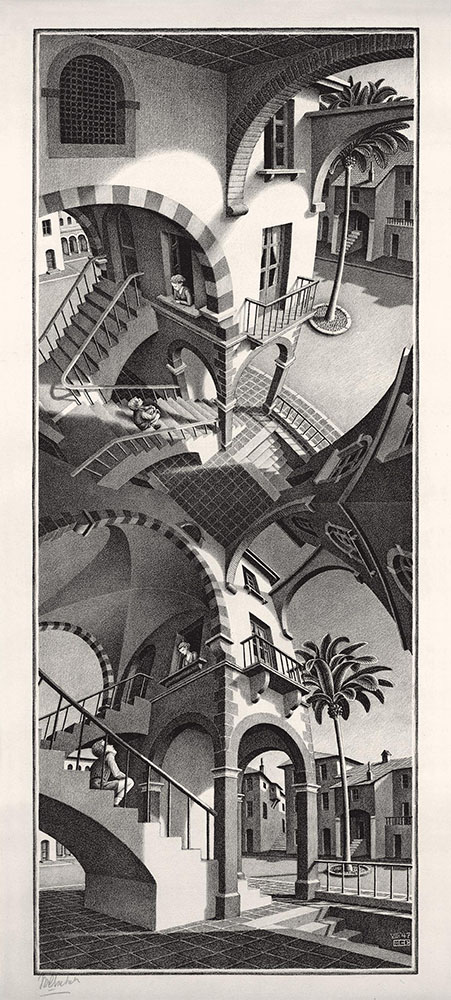
\includegraphics{img_074.jpg}
\caption[上和下,艾舍尔作。]
  {上和下,艾舍尔作(石版画,1947)。}
\end{figure}

\item[阿基里斯]我想让你从塔楼顶上观赏一下美景。

\item[乌龟]噢,那好极了。

\dnote{(他们走近了那个男孩。男孩先是好奇地瞧着他们,然后对那个年轻女人说了句什么——两人“哧哧”地笑起来。阿基里斯和乌龟并没有走上男孩坐着的楼梯,而是向左拐,沿着一段通向一座小木门的短楼梯走了下去。)}

\item[阿基里斯]我们可以从这里进去。跟着我。

\dnote{(阿基里斯推开了门,两人走进去,开始攀登塔内很陡的螺旋形楼梯。)}

\item[乌龟]\dlnote{(微微有些气喘)}作这类运动我可有点不是材料。我们还得走多久?

\item[阿基里斯]没有几段楼梯了……不过我有个想法。你干嘛非要在楼梯的正面走,你何不在反面走呢?

\item[乌龟]在反面怎么走?

\item[阿基里斯]你只消手上抓紧点,然后爬转到反面去——那面有足够的空间供你活动的。你会发现,在这些台阶的上面走和下面走是一回事……

\item[乌龟]\dlnote{(小心莫翼地爬过去)}我做得对吗?

\item[阿基里斯]就这样。

\item[乌龟]\dlnote{(声音有点变小)}喂——这个小花招真把我搞懵了,我现在应该沿着楼梯向上走还是沿着楼梯向下走?

\item[阿基里斯]同刚才的方向一样。在你那面是下楼梯,在我这面就是上楼梯。

\item[乌龟]你是不是想说我下楼梯也可以到达塔楼顶?

\item[阿基里斯]我不敢说,不过这也许是行得通的……

\dnote{(于是阿基里斯在一面往上,乌龟在另一面往下,同时沿着螺旋形的楼梯绕了起来。不久,他们都走到了楼梯的尽头。)}

现在用不着这个窍门了,龟兄,这面来——我拉你翻上来。

\dnote{(他伸手去拉乌龟,把他拽回楼梯的另一面。)}

\item[乌龟]谢谢。从反面上来倒容易些。

\dnote{(他们走上屋顶,鸟瞰全城。)}

这儿真美。阿基,我很高兴你把我带上来——也许我该说带下来。

\item[阿基里斯]我料到你会喜欢的。

\item[乌龟]我一直在想那个古怪的电话。我觉得现在明白些了。

\item[阿基里斯]是吗?跟我说说好吗?

\item[乌龟]行啊。你是不是跟我一样觉得“放在其引文形式后面”这个短语里有些叫人回味的东西?

\item[阿基里斯]有点儿,是的——很有一点。

\item[乌龟]你能想象什么东西被放在其引文后面吗?

\item[阿基里斯]我觉得我能想象出毛主席步入一间宴会厅的情景,那里悬挂着一幅大横幅,上面写着他著作的引文。这样就有了站在其引文后面的毛主席了。

\item[乌龟]这倒是个富有想象力的例子。不过假定我们把“放在……后面”的意思限制在仅指一些文字在纸上的先后次序,而不是这种煞费苦心地想出来的步入宴会厅的情景。

\item[阿基里斯]好吧。不过你说的“引文”到底是什么意思呢?

\item[乌龟]当你讨论一个词或一个短语时,根据惯例,要把它放在一对引号之内,比如,我们可以说:
\begin{block}
“哲学家”这个词有三个单字。
\end{block}
这里,我把“哲学家”放在引号之内,以表明我们说的是“哲学家”这个词,而不是某个有血有肉的哲学家本人。这就是所谓的“使用-谈论之别”。

\item[阿基里斯]噢?

\item[乌龟]我来解释一下,假如我对你说:
\begin{block}
哲学家挣大钱。
\end{block}
那么我是在“使用”这个词,从而在你心目中制造出一个目光睿智的哲人揣着个鼓鼓囊囊的大钱包的形象。可是当我把这个词——或随便什么词——加上引号时,我就抽去了它的含义和内涵,只剩下纸上的一些符号,或者说只剩下几个音节。这就叫“谈论”。除了铅字的形状以外,这个词的其它特点都无足轻重——它可能有的任何涵义都被抽掉了。

\item[阿基里斯]这叫我想起把小提琴当苍蝇拍来使用——或者我该说“谈论”?有关小提琴的一切,除了它是固体以外,一概不重要——它所具有的任何用途、功能都被抽掉了。我看苍蝇恐怕也能如此处理。

\item[乌龟]这倒是对使用—谈论之别的一个合理推广,即使有点不太正统。不过我现在要你想想一件事物放在它自身的引文形式后面的现象。

\item[阿基里斯]那好吧。你看这个行吗?
\begin{block}
“挺棒”挺棒。
\end{block}

\item[乌龟]不错,再想一个。

\item[阿基里斯]好吧。
\begin{block}
“‘咣当’不是我所见过的书名”“咣当”不是我所见过的书名。
\end{block}

\item[乌龟]这个例子稍加修改就能变成一个很有意思的典型。只消去掉“咣当”就行了。

\item[阿基里斯]真的吗?我来看看这会是什么。这一来就成了
\begin{block}
“不是我所见过的书名”不是我所见过的书名。
\end{block}

\item[乌龟]瞧,你造了一个句子。

\item[阿基里斯]是这样。这是个有关“不是我所见过的书名”这个短语的句子,是个很糟的句子。

\item[乌龟]怎么叫糟呢?

\item[阿基里斯]因为它没什么意义。我再给你造一个:
\begin{block}
“总是不了了之”总是不了了之。
\end{block}
这是什么意思?说真的,这是一种糟糕透顶的文字游戏。

\item[乌龟]我不这么想。依我看,这倒是个重要的素材。事实上,这种把一个短语放在其引文形式后面的办法极其重要,以至于我觉得该给它起个名字才好。

\item[阿基里斯]那你准备用什么名字来增加这种蠢行的尊严呢?

\item[乌龟]我想称它为“㧟摁一个短语”㧟摁一个短语。

\item[阿基里斯]“㧟摁”?这是什么词?

\item[乌龟]要是我没数错的话,这是个双音节词。

\item[阿基里斯]我是问你为什么偏要挑这么两个字,把它们按这种顺序组合起来?

\item[乌龟]哦,这回我弄懂你问我“这是什么词”的意思了。答案是:一位名叫威拉德·范·奥尔曼·蒯恩的哲学家发明了这种办法。所以我就以他名字的谐音来命名了。但是我没法做更多的解释了。至于为什么他的名字是这么两个字——更不用说为什么要按这个顺序排列了——我无可奉告。不过我倒很愿意讲点——

\item[阿基里斯]不必麻烦了!我其实也并不想知道有关蒯恩这个名字的一切事情。不管怎么说,我现在倒是知道该如何去㧟摁一个短语了。这挺好玩的。下面就是一个被㧟摁了的短语:
\begin{block}
“是个残句子”是个残句子。
\end{block}
它虽然挺糟,但我们仍然很喜欢它。拿一个残句子来,一㧟摁,瞧,就得到一个整句子!这回还是个真句子。

\item[乌龟]㧟摁一下“是个有所欠缺的国王”这一短语怎么样?

\item[阿基里斯]一个有所欠缺的国王会是——

\item[乌龟]当然是不太称职。你别往旁边岔,咱们先㧟摁了再说。

\item[阿基里斯]我来㧟摁这个短语,是吗?那好——
\begin{block}
“是个有所欠缺的国王”是个有所欠缺的国王。
\end{block}

依我看,兴许说“国王”不如说“句子”更有意义些。得了,再给我一个。

\item[乌龟]好吧——那就再来一个吧。你试试这个:
\begin{block}
“被㧟摁时得到一首乌龟情歌”
\end{block}

\item[阿基里斯]这费不了什么劲儿……你听我念这次㧟摁的结果:
\begin{block}
“被㧟摁时得到一首乌龟情歌”被㧟摁时得到一首乌龟情歌。
\end{block}

嗯嗯嗯……这里有点什么蹊跷。噢,我明白了!这个句子在说它自己!你说呢?

\item[乌龟]你这是什么意思?句子可不会说话。

\item[阿基里斯]是不会说话。不过它们都要谈到点什么——而这个句子则是直截了当地——无歧义也无偏差地——谈到它自身!你就不得不转过头来回想一下㧟摁到底是怎么回事了。

\item[乌龟]我看不出它在说有关它自己的什么事情。它什么时候说过“我”或“本句子”之类的话?

\item[阿基里斯]哎,你故意装傻吧?其美妙之处就在于它说了自己而又不必直接挑明!

\item[乌龟]那好吧,对我这么个笨朋友,你能不能详细讲讲?

\item[阿基里斯]嗯,你真是个满腹狐疑的乌龟……行啊,让我想想……假定我造出一个句子。就把它叫“句子J”吧,因为它里面有个空位——或者说“洞眼”。

\item[乌龟]比如说?

\item[阿基里斯]比如说
\begin{block}
\underline{\kern2\ccwd},被㧟摁时,得到一支乌龟情歌”。
\end{block}

那么句子J的论题就依赖于我们如何填充这个空位。不过只要空位上该填的东西选好了,它也就确定了:它就是㧟摁这个空位所得到的那个短语。由于它是由一个㧟摁行为生成的,我们就把它叫做“句子K”。

\item[乌龟]这回懂了。如果空位里的句子是“总是被到处宣扬”,那句子K就必定是
\begin{block}
“总是被到处宣扬”总是被到处宣扬。
\end{block}

\item[阿基里斯]是的,句子J宣称(至于是真是假,我并不知道):句子K是一首乌龟情歌。无论如何,句子J在这里并没有说到它自己,而是说句子K。这些我们都是一致的吧?

\item[乌龟]不管怎么说,让我们也都同意这是一首优美的歌曲吧。

\item[阿基里斯]不过此刻我要另造一个东西来填空,那就是:
\begin{block}
“被㧟摁时得到一首乌龟情歌”
\end{block}

\item[乌龟]啊,天哪,你开始复杂起来了。我希望这一切别太高深得让我摸不着头脑。

\item[阿基里斯]噢,别担心——你肯定能明白。由于这样选择,句子K就变成
\begin{block}
“被㧟摁时得到一首乌龟情歌”被㧟摁时得到一首乌龟情歌。
\end{block}

\item[乌龟]噢,你这个滑头,我明白了。这样一来句子K就恰好和句子J一样了。

\item[阿基里斯]由于句子K总是句子J的论题,这就有了一个圈,所有J就反过来指向自己。不过你看到了,自指乃是一种巧合。而通常的情形是句子J与句子K彼此完全不同,但随着对句子J中空位的恰当选择,㧟摁就能给你变出这种戏法来。

\item[乌龟]噢,好机巧啊。真奇怪,我自己怎么就从来没想到过这些呢?那你来说说,下面这个句子是不是个自指的?
\begin{block}
“由六个字组成”由六个字组成。
\end{block}

\item[阿基里斯]嗯嗯嗯……我恐怕说不好。你刚才给出的这个句子其实不是关于它自己的,而是关于“由六个字组成”这个短语的。当然,不管怎么说这个短语是该句子的一部分……

\item[乌龟]那么这个句子就是在谈论自己的某个部分了——这会怎么样呢?

\item[阿基里斯]这也可以叫做自指吗?

\item[乌龟]依我看,这还远不是自指。不过你也别太为这些鬼事烦恼,以后你会有充裕的时间去进一步思考它们的。

\item[阿基里斯]我会吗?

\item[乌龟]你会的。而眼下你何不试着㧟摁一下“放在其引文形式后面得到假句子”这个短语呢?

\item[阿基里斯]我明白你发现什么了——就是先前那个古怪电话。㧟摁它就得到:
\begin{block}
“放在其引文形式后面得到假句子”放在其引文形式后面得到假句子。
\end{block}

这正是那个电话里所说的!只是在他说话时我没弄清什么地方有引号!真是句混帐话。说这种话的人都该进监狱。

\item[乌龟]为什么?

\item[阿基里斯]它太让我难受了。它和前面的那些例子不一样,我这回弄不清它到底是真句子还是假句子。我越是使劲想就越理不清楚。我的头都晕了。我真想知道编出这种东西的人得了哪种神经病,居然夜里拿它去折磨无辜的人。

\item[乌龟]我也不清楚……得了,我们该下去了吧?

\item[阿基里斯]用不着下去——我们已经在地面上了。进去吧——进去你就明白了。

\dnote{(他们走进塔楼,来到一个小木门前)}

从这里就能走出去,跟我来。

\item[乌龟]你能肯定吗?我可不想从三楼上掉下去把背壳摔裂。

\item[阿基里斯]我还能骗你?

\dnote{(他打开门,在他们前面坐着同一个男孩,正和同一个年轻女人说话,周围的一切也都一模一样。阿基里斯和乌龟走上看上去和他们进塔楼时走下的那段楼梯完全一样的楼梯,并且发现他们自己是站在一个看上去和他们最初所进的院子完全一样的院子中。)}

谢谢你澄清了那个古怪的电话,龟兄。

\item[乌龟]也要谢谢你,阿基,这次散步十分愉快。希望我们很快还能见面。

\end{dialogue}

\end{dialog}
